\chapter{Installation}
\label{chap:installation}

\section{Install Our Plugin for Enterprise Architect (EA)}
\begin{enumerate}
\item[$\blacktriangleright$] Download and install EA (Fig.~
\ref{fig_enterpriseArchitextHomepage}) 
\item[] Go to \url{http://www.sparxsystems.com.au/} to get a free 30 day trial.
\begin{figure}[!h]
	\centering
  
\includegraphics[width=0.7\textwidth]{pics/ea_download.png}
	\caption{Download Enterprise Architect}
	\label{fig_enterpriseArchitextHomepage}
\end{figure} 
\item[$\blacktriangleright$] Install our EA-Plugin (Fig.~
\ref{fig_eaPluginWizard})
\item[] Download zip from
\url{http://www.moflon.org/fileadmin/download/moflon-ide/eclipse-plugin/ea-ecore-addin/ea-ecore-addin.zip},
unpack, and run setup.exe
\begin{figure}[!h]
	\centering
  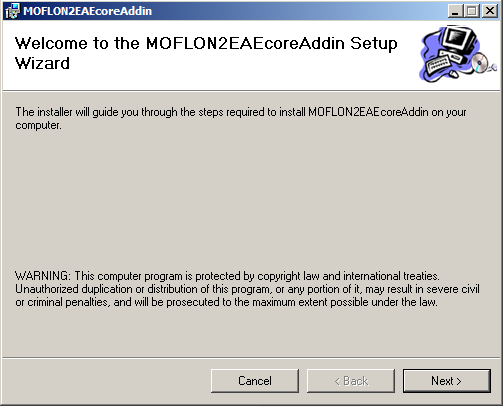
\includegraphics[width=0.3\textwidth]{pics/eaplugin_install.png}
	\caption{Install our plugin for EA.}
	\label{fig_eaPluginWizard}
\end{figure}
\end{enumerate}

\section{Install Our Plugin for Eclipse}
\begin{enumerate}
\item[$\blacktriangleright$] Download and install Eclipse for Modeling
``Eclipse Modeling Tools (includes Incubating components)''
(Fig.~\ref{fig_downloadModelingPackage}) from:\\  
\url{http://www.eclipse.org/downloads/packages/}
\begin{figure}[!h]
	\centering
  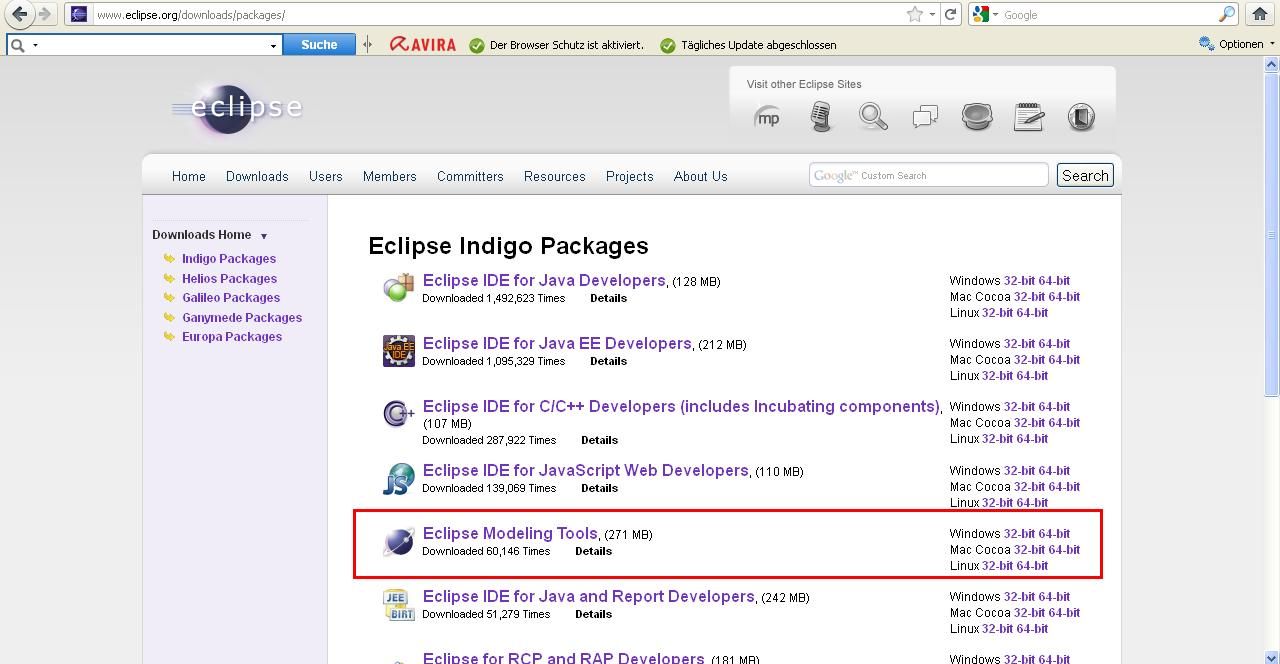
\includegraphics[width=0.7\textwidth]{pics/eclipse_modelingpackage.png}
	\caption{Download Eclipse Modeling Tools.}
	\label{fig_downloadModelingPackage}
\end{figure}
\item[$\blacktriangleright$] Install our Eclipse Plugin from the following
update site\footnote{For a detailed tutorial on how to install Eclipse and
Eclipse Plugins please refer to
\url{http://www.vogella.de/articles/Eclipse/article.html}} 
\footnote{Please note: Calculating requirements and dependencies when installing
the plugin might take quite a while depending on your internet connection.}:
\url{http://www.moflon.org/fileadmin/download/moflon-ide/eclipse-plugin/update-site2}
\end{enumerate}

\newpage

\section{Get a Simple Demo Running}

\begin{enumerate}
\item[$\blacktriangleright$] Go to ``Window/Open Perspective/Other\ldots'' and
choose Moflon (Fig.~\ref{fig_eclipse}).
\begin{figure}[!h]
	\centering
  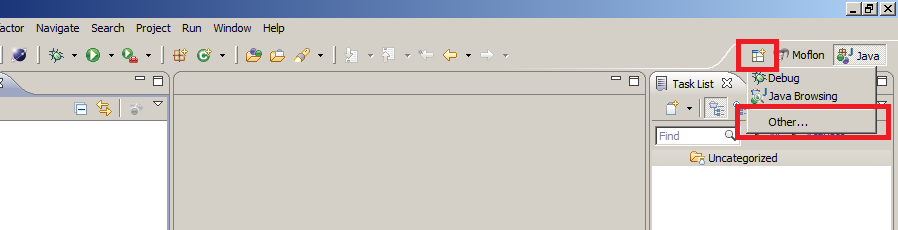
\includegraphics[width=0.7\textwidth]{pics/eclipse_firststart.png}
	\caption{Choose the Moflon Perspective.}
	\label{fig_eclipse}
\end{figure}

\item[$\blacktriangleright$] In the toolbar a new action set should have
appeared. Choose ``New Metamodel'' (Fig.~\ref{fig_eclipseNewMetamodel}).
The button with an ``L" shows you our logfile (important input for us if
something goes wrong!).
\begin{figure}[!h]
	\centering
  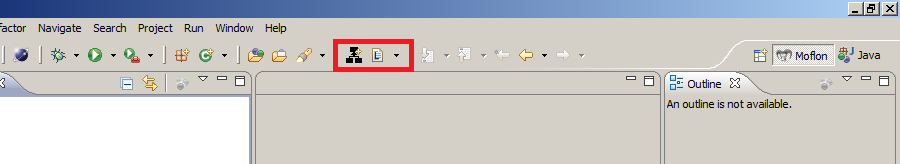
\includegraphics[width=0.8\textwidth]{pics/eclipse_metamodelButton.png}
	\caption{Eclipse New Metamodel}
	\label{fig_eclipseNewMetamodel}
\end{figure}

\item[$\blacktriangleright$] Enter ``Demo'' as the name of the new metamodel
project and confirm. 
An empty EA project file ``Demo.eap'' will be
created in a new project with a certain project structure
according to our conventions.

\newpage

%\item[$\blacktriangleright$] Choose working sets as your top level element in
%the package explorer (Fig.~\ref{fig_eclipseWorkingsets}).
%We work a lot with working sets and use them to structure the workspace in
%Eclipse.
%\begin{figure}[!h]
%	\centering
%  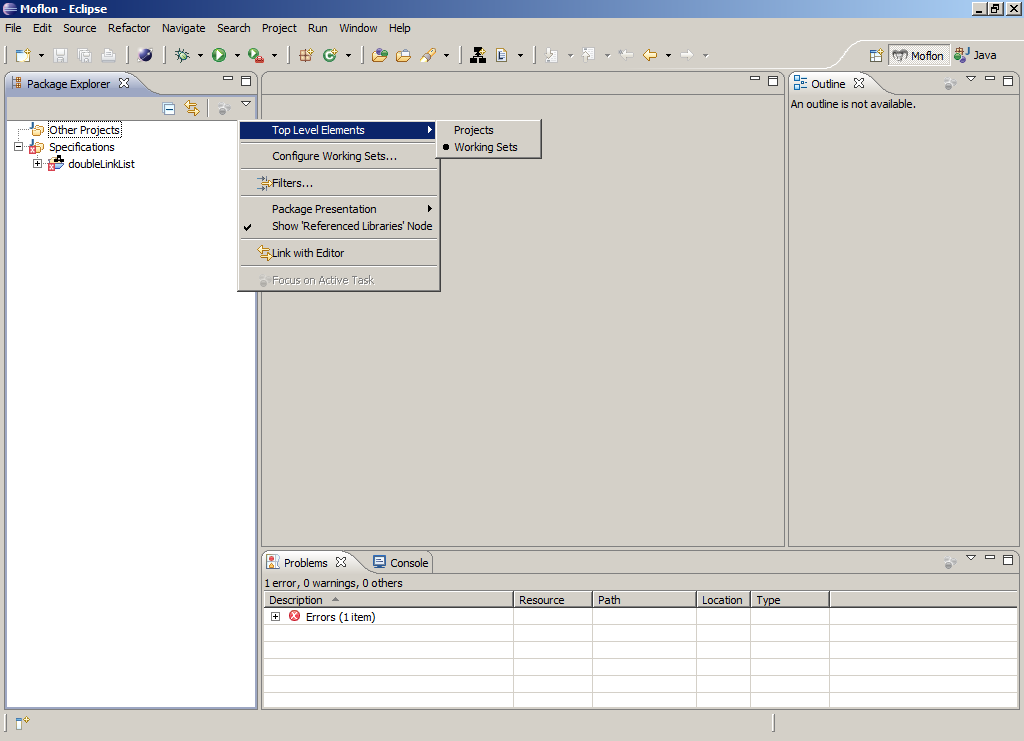
\includegraphics[width=0.6\textwidth]{pics/eclipse_workingsets.png}
%	\caption{Choose Working Sets as Top Level Elements.}
%	\label{fig_eclipseWorkingsets}
%\end{figure}

\item[$\blacktriangleright$] Open the newly created project and replace the
``Demo.eap'' file with the Demo.eap that you will find in the
same folder as this tutorial. 
This EA file already contains our simple demo project.

\item[$\blacktriangleright$] Double click ``Demo.eap'' to start EA.
Please choose ``Ultimate" when starting EA for the first time.

\item[$\blacktriangleright$] In EA, choose ``Add-Ins/MOFLON::Ecore Addin/Export
all to Workspace'' (Fig.~\ref{fig_ea}).
\begin{figure}[!h]
	\centering
  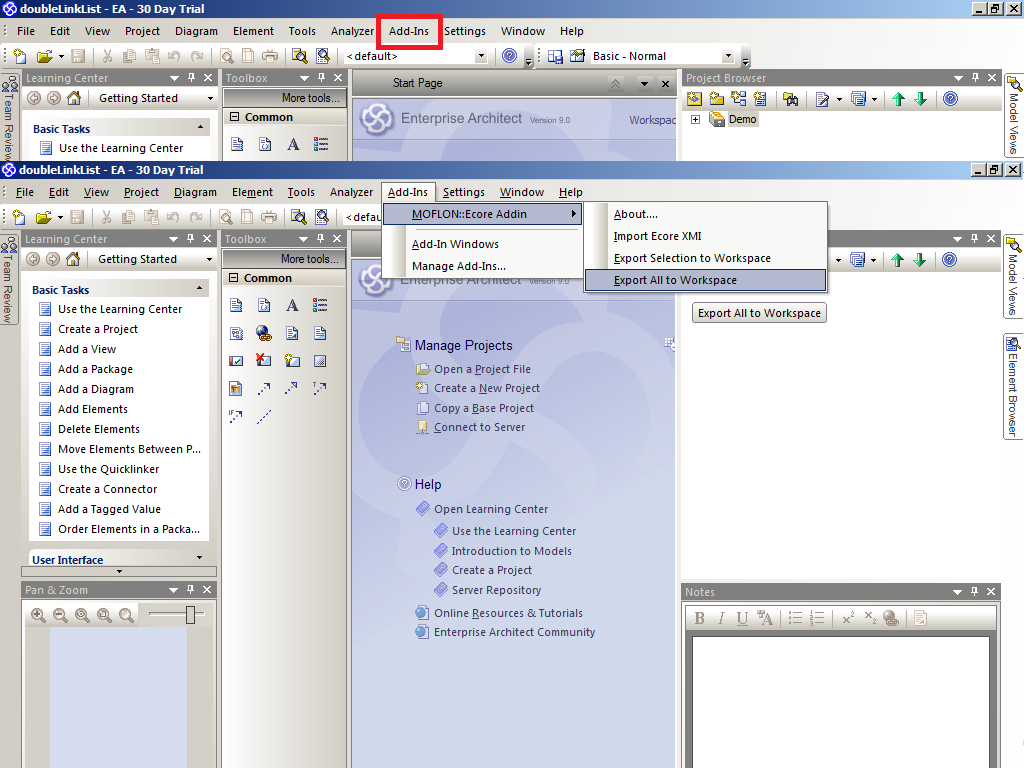
\includegraphics[width=0.65\textwidth]{pics/ea_firststart.png}
	\caption{Export from EA with our plugin.}
	\label{fig_ea}
\end{figure}

\newpage

\item[$\blacktriangleright$] Switch back to Eclipse, choose your Metamodel
project and press F5 to refresh.
The export from EA places all required files in a hidden folder in the
project, and refreshing triggers a build process that invokes our different
code generators automatically.
You should be able to monitor the progress in the lower right corner
(Fig.~\ref{fig_eclipsebuilding}).  
Pressing the symbol opens a monitor view that gives more details of the build
process. 
\begin{figure}[!h]
	\centering
  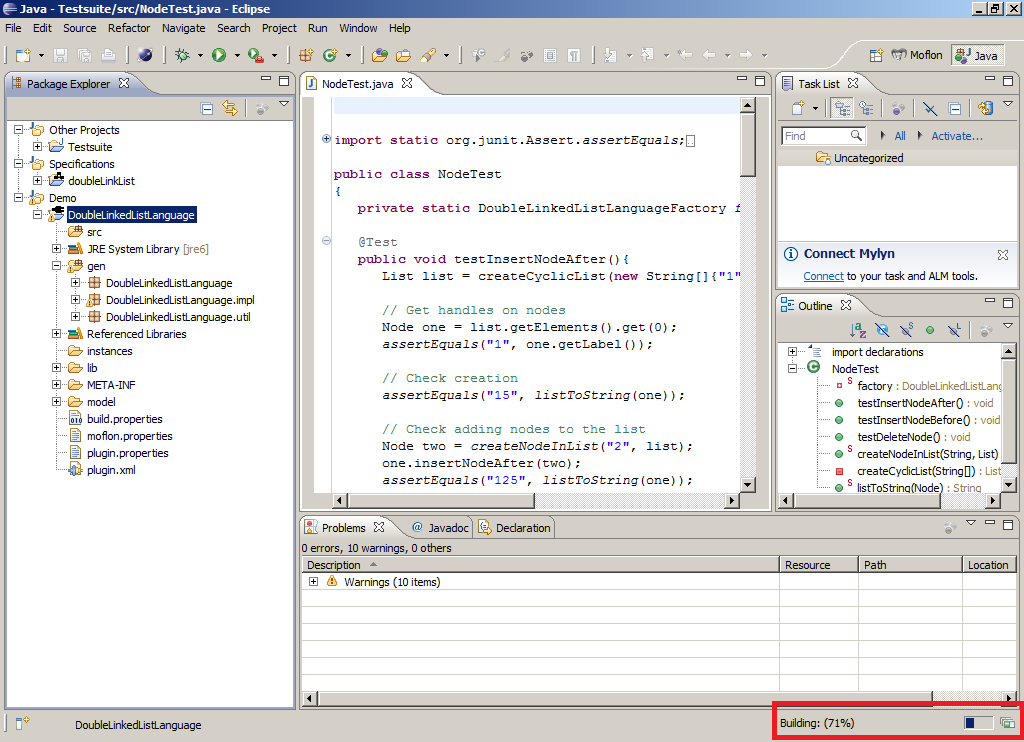
\includegraphics[width=0.6\textwidth]{pics/eclipse_building.png}
	\caption{Automatically building the workspace after a refresh.}
	\label{fig_eclipsebuilding}
\end{figure}
\end{enumerate}

\section{Validate Your Installation with JUnit}

\begin{enumerate}
\item[$\blacktriangleright$] Go to ``File/Import/General/Existing Projects
into Workspace'' (Fig.~\ref{fig_eclipseTestsuiteImport}) and choose the
Testsuite project that is also in the same folder as this tutorial. 
\begin{figure}[!h]
	\centering
  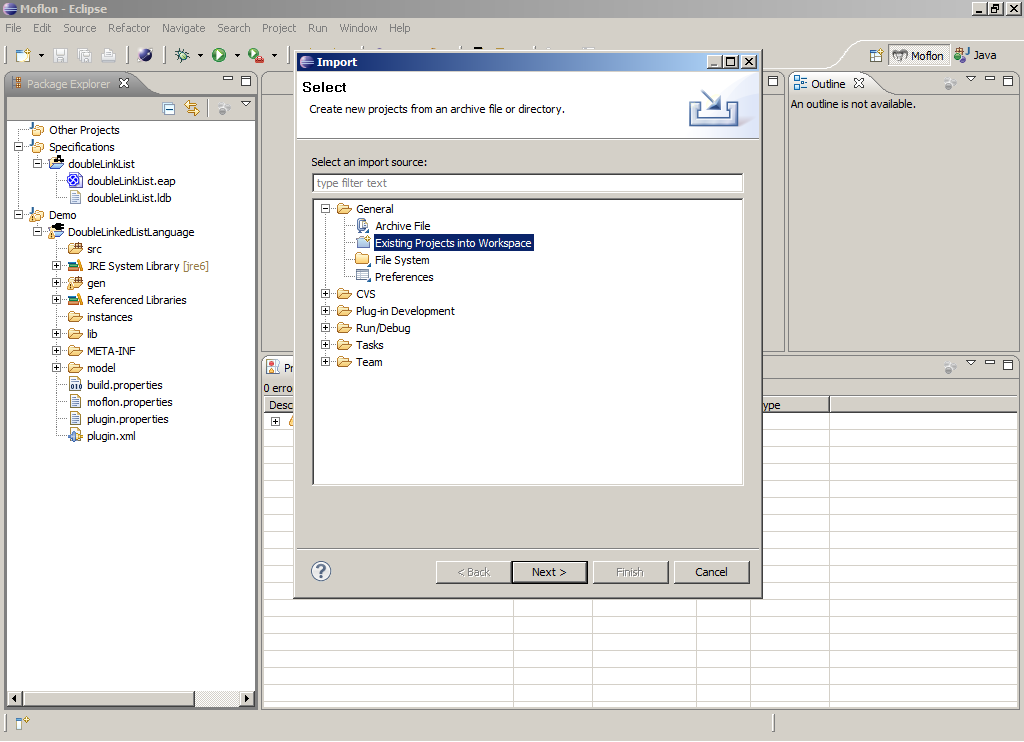
\includegraphics[width=0.6\textwidth]{pics/eclipse_testsuitimport.png}
	\caption{Import our Testsuite as an existing project.}
	\label{fig_eclipseTestsuiteImport}
\end{figure}

\newpage 

\item[] At this point, your workspace should resemble
Fig.~\ref{fig_eclipsepackageexplorer}.
\begin{figure}[!h]
	\centering
  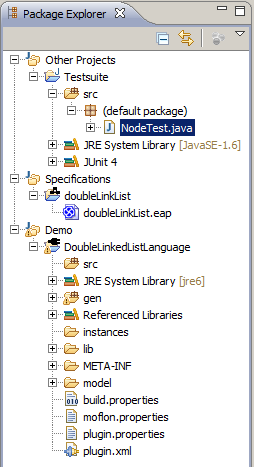
\includegraphics[width=0.2\textwidth]{pics/eclipse_packageexplorer.png}
	\caption{Workspace in Eclipse.}
	\label{fig_eclipsepackageexplorer}
\end{figure}

\item[$\blacktriangleright$] Right-click on the Testsuite project and select
``Run as/JUnit Test''.
Congratulations!  If you see a green bar  (Fig.~\ref{fig_eclipsetestsuiterun}),
then everything has been set-up correctly and you are now ready to start
metamodelling!
\begin{figure}[!h]
	\centering
  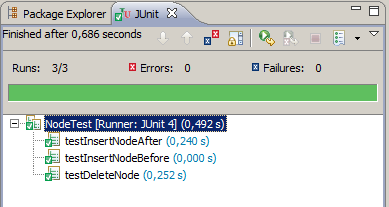
\includegraphics[width=0.2\textwidth]{pics/eclipse_testsuiterun.png}
	\caption{All's well that ends well\ldots}
	\label{fig_eclipsetestsuiterun}
\end{figure}
\end{enumerate}